\documentclass{article}\usepackage[]{graphicx}\usepackage[]{color}
%% maxwidth is the original width if it is less than linewidth
%% otherwise use linewidth (to make sure the graphics do not exceed the margin)
\makeatletter
\def\maxwidth{ %
  \ifdim\Gin@nat@width>\linewidth
    \linewidth
  \else
    \Gin@nat@width
  \fi
}
\makeatother

\definecolor{fgcolor}{rgb}{0.345, 0.345, 0.345}
\newcommand{\hlnum}[1]{\textcolor[rgb]{0.686,0.059,0.569}{#1}}%
\newcommand{\hlstr}[1]{\textcolor[rgb]{0.192,0.494,0.8}{#1}}%
\newcommand{\hlcom}[1]{\textcolor[rgb]{0.678,0.584,0.686}{\textit{#1}}}%
\newcommand{\hlopt}[1]{\textcolor[rgb]{0,0,0}{#1}}%
\newcommand{\hlstd}[1]{\textcolor[rgb]{0.345,0.345,0.345}{#1}}%
\newcommand{\hlkwa}[1]{\textcolor[rgb]{0.161,0.373,0.58}{\textbf{#1}}}%
\newcommand{\hlkwb}[1]{\textcolor[rgb]{0.69,0.353,0.396}{#1}}%
\newcommand{\hlkwc}[1]{\textcolor[rgb]{0.333,0.667,0.333}{#1}}%
\newcommand{\hlkwd}[1]{\textcolor[rgb]{0.737,0.353,0.396}{\textbf{#1}}}%
\let\hlipl\hlkwb

\usepackage{framed}
\makeatletter
\newenvironment{kframe}{%
 \def\at@end@of@kframe{}%
 \ifinner\ifhmode%
  \def\at@end@of@kframe{\end{minipage}}%
  \begin{minipage}{\columnwidth}%
 \fi\fi%
 \def\FrameCommand##1{\hskip\@totalleftmargin \hskip-\fboxsep
 \colorbox{shadecolor}{##1}\hskip-\fboxsep
     % There is no \\@totalrightmargin, so:
     \hskip-\linewidth \hskip-\@totalleftmargin \hskip\columnwidth}%
 \MakeFramed {\advance\hsize-\width
   \@totalleftmargin\z@ \linewidth\hsize
   \@setminipage}}%
 {\par\unskip\endMakeFramed%
 \at@end@of@kframe}
\makeatother

\definecolor{shadecolor}{rgb}{.97, .97, .97}
\definecolor{messagecolor}{rgb}{0, 0, 0}
\definecolor{warningcolor}{rgb}{1, 0, 1}
\definecolor{errorcolor}{rgb}{1, 0, 0}
\newenvironment{knitrout}{}{} % an empty environment to be redefined in TeX

\usepackage{alltt}

\usepackage{amsmath, amssymb}
\usepackage{graphicx}
\usepackage{hyperref}
\IfFileExists{upquote.sty}{\usepackage{upquote}}{}
\begin{document}

\title{Pol Sci 630:  Problem Set 10: Functional Form, Endogeneity, Power}

\author{Prepared by: Anh Le (\href{mailto:anh.le@duke.edu}{anh.le@duke.edu})}

\date{Due Date: Nov 9 (Beginning of Class)}

\maketitle

\section{Functional specification}

There's a famous dataset called the Anscombe quartet. You load it in R like so:

\begin{knitrout}
\definecolor{shadecolor}{rgb}{0.969, 0.969, 0.969}\color{fgcolor}\begin{kframe}
\begin{alltt}
\hlkwd{head}\hlstd{(anscombe)}
\end{alltt}
\begin{verbatim}
##   x1 x2 x3 x4   y1   y2    y3   y4
## 1 10 10 10  8 8.04 9.14  7.46 6.58
## 2  8  8  8  8 6.95 8.14  6.77 5.76
## 3 13 13 13  8 7.58 8.74 12.74 7.71
## 4  9  9  9  8 8.81 8.77  7.11 8.84
## 5 11 11 11  8 8.33 9.26  7.81 8.47
## 6 14 14 14  8 9.96 8.10  8.84 7.04
\end{verbatim}
\end{kframe}
\end{knitrout}

\subsection{Explore Anscombe}

There are 4 pairs of $x$ and $y$. Run 4 regressions of y on x. Check out the regression result. A bit late for Halloween, but what spooky thing do you notice?

Then plot the data.

\textbf{Solution}

\begin{knitrout}
\definecolor{shadecolor}{rgb}{0.969, 0.969, 0.969}\color{fgcolor}\begin{kframe}
\begin{alltt}
\hlstd{(m1} \hlkwb{<-} \hlkwd{lm}\hlstd{(y1} \hlopt{~} \hlstd{x1,} \hlkwc{data} \hlstd{= anscombe))}
\end{alltt}
\begin{verbatim}
## 
## Call:
## lm(formula = y1 ~ x1, data = anscombe)
## 
## Coefficients:
## (Intercept)           x1  
##      3.0001       0.5001
\end{verbatim}
\begin{alltt}
\hlstd{(m2} \hlkwb{<-} \hlkwd{lm}\hlstd{(y2} \hlopt{~} \hlstd{x2,} \hlkwc{data} \hlstd{= anscombe))}
\end{alltt}
\begin{verbatim}
## 
## Call:
## lm(formula = y2 ~ x2, data = anscombe)
## 
## Coefficients:
## (Intercept)           x2  
##       3.001        0.500
\end{verbatim}
\begin{alltt}
\hlstd{(m3} \hlkwb{<-} \hlkwd{lm}\hlstd{(y3} \hlopt{~} \hlstd{x3,} \hlkwc{data} \hlstd{= anscombe))}
\end{alltt}
\begin{verbatim}
## 
## Call:
## lm(formula = y3 ~ x3, data = anscombe)
## 
## Coefficients:
## (Intercept)           x3  
##      3.0025       0.4997
\end{verbatim}
\begin{alltt}
\hlstd{(m4} \hlkwb{<-} \hlkwd{lm}\hlstd{(y4} \hlopt{~} \hlstd{x4,} \hlkwc{data} \hlstd{= anscombe))}
\end{alltt}
\begin{verbatim}
## 
## Call:
## lm(formula = y4 ~ x4, data = anscombe)
## 
## Coefficients:
## (Intercept)           x4  
##      3.0017       0.4999
\end{verbatim}
\begin{alltt}
\hlkwd{par}\hlstd{(}\hlkwc{mfrow}\hlstd{=}\hlkwd{c}\hlstd{(}\hlnum{2}\hlstd{,}\hlnum{2}\hlstd{))}
\hlkwd{plot}\hlstd{(y1} \hlopt{~} \hlstd{x1,} \hlkwc{data} \hlstd{= anscombe)}
\hlkwd{plot}\hlstd{(y2} \hlopt{~} \hlstd{x2,} \hlkwc{data} \hlstd{= anscombe)}
\hlkwd{plot}\hlstd{(y3} \hlopt{~} \hlstd{x3,} \hlkwc{data} \hlstd{= anscombe)}
\hlkwd{plot}\hlstd{(y4} \hlopt{~} \hlstd{x4,} \hlkwc{data} \hlstd{= anscombe)}
\end{alltt}
\end{kframe}
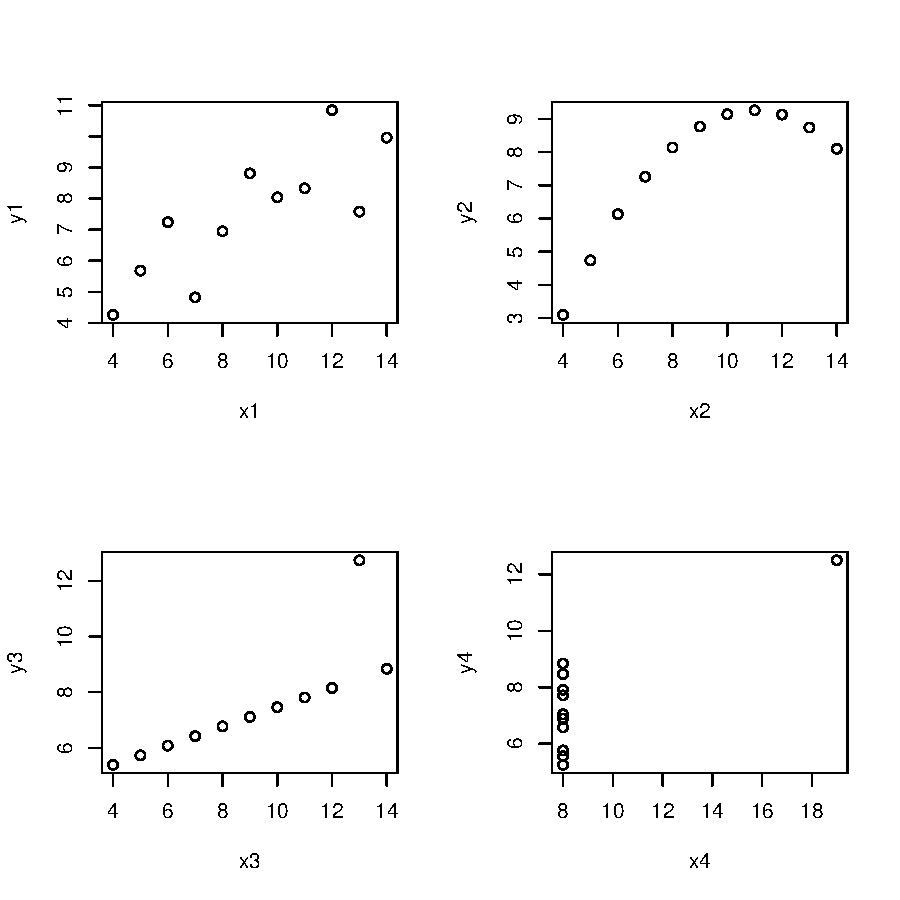
\includegraphics[width=\maxwidth]{figure/unnamed-chunk-2-1} 
\begin{kframe}\begin{alltt}
\hlkwd{par}\hlstd{(}\hlkwc{mfrow}\hlstd{=}\hlkwd{c}\hlstd{(}\hlnum{1}\hlstd{,}\hlnum{1}\hlstd{))}
\end{alltt}
\end{kframe}
\end{knitrout}

The four regression models have exactly the same coefficients, standard errors, p-value, R-square (!). But the pattern of the data looks very different. A good lesson about why we visualize data and don't run regression blindly.

\subsection{Ramsey RESET}

Use Ramsey RESET on the 4 models to check. Which kind of functional misclassification can it catch?

\textbf{Solution}

\begin{knitrout}
\definecolor{shadecolor}{rgb}{0.969, 0.969, 0.969}\color{fgcolor}\begin{kframe}
\begin{alltt}
\hlkwd{library}\hlstd{(lmtest)}
\end{alltt}


{\ttfamily\noindent\itshape\color{messagecolor}{\#\# Loading required package: zoo}}

{\ttfamily\noindent\itshape\color{messagecolor}{\#\# \\\#\# Attaching package: 'zoo'}}

{\ttfamily\noindent\itshape\color{messagecolor}{\#\# The following objects are masked from 'package:base':\\\#\# \\\#\#\ \ \ \  as.Date, as.Date.numeric}}\begin{alltt}
\hlkwd{resettest}\hlstd{(m1,} \hlkwc{power} \hlstd{=} \hlnum{2}\hlstd{,} \hlkwc{type} \hlstd{=} \hlstr{"fitted"}\hlstd{)}
\end{alltt}
\begin{verbatim}
## 
## 	RESET test
## 
## data:  m1
## RESET = 0.5318, df1 = 1, df2 = 8, p-value = 0.4866
\end{verbatim}
\begin{alltt}
\hlkwd{resettest}\hlstd{(m2,} \hlkwc{power} \hlstd{=} \hlnum{2}\hlstd{,} \hlkwc{type} \hlstd{=} \hlstr{"fitted"}\hlstd{)}
\end{alltt}
\begin{verbatim}
## 
## 	RESET test
## 
## data:  m2
## RESET = 4925000, df1 = 1, df2 = 8, p-value < 2.2e-16
\end{verbatim}
\begin{alltt}
\hlkwd{resettest}\hlstd{(m3,} \hlkwc{power} \hlstd{=} \hlnum{2}\hlstd{,} \hlkwc{type} \hlstd{=} \hlstr{"fitted"}\hlstd{)}
\end{alltt}
\begin{verbatim}
## 
## 	RESET test
## 
## data:  m3
## RESET = 0.46605, df1 = 1, df2 = 8, p-value = 0.5141
\end{verbatim}
\begin{alltt}
\hlkwd{resettest}\hlstd{(m4,} \hlkwc{power} \hlstd{=} \hlnum{2}\hlstd{,} \hlkwc{type} \hlstd{=} \hlstr{"fitted"}\hlstd{)}
\end{alltt}
\begin{verbatim}
## 
## 	RESET test
## 
## data:  m4
## RESET = 0, df1 = 1, df2 = 8, p-value = 1
\end{verbatim}
\end{kframe}
\end{knitrout}

The RESET test can only catch the second case, where there is a curvillinear relationship. This is because RESET simply adds squared terms and check whether they are important. Even though it's problematic to say the 3rd and 4th models are a good fit, RESET can't catch it.

This is to show what a test can and cannot do.

\section{Endogeneity -- Omitted Variable Bias}

\subsection{Sign the bias -- math}

Given the following data generating process (DGP)

\begin{align}
x_2 &= \delta_0 + \delta_1 x_1 + v \\
y &= \beta_0 + \beta_1 x_1 + \beta_2 x_2 + w
\end{align}

The following equation (lecture 09/26) shows what happens when we regress $y$ on $x_1$, omitting $x_2$. \textbf{Prove this equation}.

$$
y = (\beta_0 + \beta_2 \delta_0) + (\beta_1 + \beta_2 \delta_1) x_1 + (\beta_2 v + w)
$$



\textbf{Solution}

\begin{align}
y &= \beta_0 + \beta_1 x_1 + \beta_2 x_2 + w \\
&= \beta_0 + \beta_1 x_1 + \beta_2 (\delta_0 + \delta_1 x_1 + v) + w \\
&= (\beta_0 + \beta_2 \delta_0) + (\beta_1 + \beta_2 \delta_1) x_1 + (\beta_2 v + w)
\end{align}

\subsection{Sign the bias - simulation}

In the equation you proved above, the estimated coefficient for $x_1$ is $\beta_1 + \beta_2 \delta_1$, different from its true value $\beta_1$. The bias is $\beta_2\delta_1$. The sign of the bias thus depends on $\beta_2$ and $\delta_1$, as discussed in the lecture and reproduced in Table 1.

\begin{table}[]
\centering
\caption{Signing the bias}
\label{my-label}
\begin{tabular}{|l|l|l|}
\hline
               & $\beta_2 > 0$ & $\beta_2 < 0$ \\ \hline
$\delta_1 > 0$ &               &               \\ \hline
$\delta_1 < 0$ &               &               \\ \hline
\end{tabular}
\end{table}

Conduct 4 simulations with appropriate values of $\beta_2$ and $\delta_1$ corresponding to the 4 cells in the table. Show that the sign of the bias is as we learned in class.

\textbf{Solution}

We create a function that calculates the bias depending on the values of $\beta_2$ and $\delta_1$.
\begin{knitrout}
\definecolor{shadecolor}{rgb}{0.969, 0.969, 0.969}\color{fgcolor}\begin{kframe}
\begin{alltt}
\hlstd{delta1} \hlkwb{<-} \hlnum{1} \hlstd{; beta2} \hlkwb{<-} \hlnum{3} \hlcom{# These 2 are keys}

\hlstd{bias_simulation} \hlkwb{<-} \hlkwa{function}\hlstd{(}\hlkwc{beta2}\hlstd{,} \hlkwc{delta1}\hlstd{) \{}
  \hlstd{beta0} \hlkwb{<-} \hlnum{1} \hlstd{; beta1} \hlkwb{<-} \hlnum{2} \hlstd{; delta0} \hlkwb{<-} \hlnum{1} \hlcom{# These don't matters for bias sign}
  \hlstd{x2} \hlkwb{<-} \hlkwd{rnorm}\hlstd{(}\hlnum{100}\hlstd{)}
  \hlstd{x1} \hlkwb{<-} \hlstd{delta1} \hlopt{*} \hlstd{x2} \hlopt{+} \hlkwd{rnorm}\hlstd{(}\hlnum{100}\hlstd{)}
  \hlstd{y} \hlkwb{<-} \hlstd{beta0} \hlopt{+} \hlstd{beta1} \hlopt{*} \hlstd{x1} \hlopt{+} \hlstd{beta2} \hlopt{*} \hlstd{x2} \hlopt{+} \hlkwd{rnorm}\hlstd{(}\hlnum{100}\hlstd{)}

  \hlstd{estimated_beta1} \hlkwb{<-} \hlkwd{coef}\hlstd{(}\hlkwd{lm}\hlstd{(y} \hlopt{~} \hlstd{x1))[}\hlstr{"x1"}\hlstd{]}
  \hlstd{bias} \hlkwb{<-} \hlstd{estimated_beta1} \hlopt{-} \hlstd{beta1}
  \hlkwd{return}\hlstd{(bias)}
\hlstd{\}}
\end{alltt}
\end{kframe}
\end{knitrout}

We use this function to show the sign of the bias in each of the 4 cells

\begin{knitrout}
\definecolor{shadecolor}{rgb}{0.969, 0.969, 0.969}\color{fgcolor}\begin{kframe}
\begin{alltt}
\hlkwd{bias_simulation}\hlstd{(}\hlkwc{beta2} \hlstd{=} \hlnum{1}\hlstd{,} \hlkwc{delta1} \hlstd{=} \hlnum{1}\hlstd{)}
\end{alltt}
\begin{verbatim}
##        x1 
## 0.5484303
\end{verbatim}
\begin{alltt}
\hlkwd{bias_simulation}\hlstd{(}\hlkwc{beta2} \hlstd{=} \hlnum{1}\hlstd{,} \hlkwc{delta1} \hlstd{=} \hlopt{-}\hlnum{1}\hlstd{)}
\end{alltt}
\begin{verbatim}
##         x1 
## -0.5060759
\end{verbatim}
\begin{alltt}
\hlkwd{bias_simulation}\hlstd{(}\hlkwc{beta2} \hlstd{=} \hlopt{-}\hlnum{1}\hlstd{,} \hlkwc{delta1} \hlstd{=} \hlopt{-}\hlnum{1}\hlstd{)}
\end{alltt}
\begin{verbatim}
##        x1 
## 0.2718827
\end{verbatim}
\begin{alltt}
\hlkwd{bias_simulation}\hlstd{(}\hlkwc{beta2} \hlstd{=} \hlopt{-}\hlnum{1}\hlstd{,} \hlkwc{delta1} \hlstd{=} \hlnum{1}\hlstd{)}
\end{alltt}
\begin{verbatim}
##       x1 
## -0.66955
\end{verbatim}
\end{kframe}
\end{knitrout}

We confirm that whenever $\beta_2$ and $\delta_1$ are of opposite sign, we have negative bias.

\section{Power calculation}

In this exercise we practice power calculation for the simplest experiment setup.

Assume that our binary treatment has an effect size of 2 on the outcome, as follows:

$$
\begin{aligned}
y &= 1 + 2 \times \text{Treatment} + u \\
u &\sim Normal(mean = 1, sd = 10) \\
\end{aligned}
$$

In our experiment, we randomly assigned $n$ experimental units into 2 groups, treated and control, i.e. treatment = 1 and treatment = 0. Calculate the power of our experiment (i.e. the probability that we can reject the null of zero treatment effect) for different values of the sample size $n$.

The end product I want to see is a graph with $n$ on the x-axis and power on the y-axis. How big must your sample size be to get a power of 0.8?

\textbf{Solution}

We first create a function that takes a value of n and calculate the power.
\begin{knitrout}
\definecolor{shadecolor}{rgb}{0.969, 0.969, 0.969}\color{fgcolor}\begin{kframe}
\begin{alltt}
\hlstd{power_sim} \hlkwb{<-} \hlkwa{function}\hlstd{(}\hlkwc{n}\hlstd{) \{}
  \hlstd{number_of_simulations} \hlkwb{<-} \hlnum{100}
  \hlstd{pvalues} \hlkwb{<-} \hlkwd{rep}\hlstd{(}\hlnum{NA}\hlstd{, number_of_simulations)}
  \hlkwa{for} \hlstd{(i} \hlkwa{in} \hlnum{1}\hlopt{:}\hlstd{number_of_simulations) \{}
    \hlstd{treatment} \hlkwb{<-} \hlkwd{sample}\hlstd{(}\hlkwd{c}\hlstd{(}\hlnum{0}\hlstd{,} \hlnum{1}\hlstd{),} \hlkwc{size} \hlstd{= n,} \hlkwc{replace} \hlstd{=} \hlnum{TRUE}\hlstd{)}
    \hlstd{y} \hlkwb{<-} \hlnum{1} \hlopt{+} \hlnum{2} \hlopt{*} \hlstd{treatment} \hlopt{+} \hlkwd{rnorm}\hlstd{(n,} \hlkwc{mean} \hlstd{=} \hlnum{1}\hlstd{,} \hlkwc{sd} \hlstd{=} \hlnum{10}\hlstd{)}
    \hlstd{pvalues[i]} \hlkwb{<-} \hlkwd{coef}\hlstd{(}\hlkwd{summary}\hlstd{(}\hlkwd{lm}\hlstd{(y} \hlopt{~} \hlstd{treatment)))[}\hlnum{2}\hlstd{,} \hlnum{4}\hlstd{]}
  \hlstd{\}}
  \hlkwd{mean}\hlstd{(pvalues} \hlopt{<} \hlnum{0.05}\hlstd{)}
\hlstd{\}}
\end{alltt}
\end{kframe}
\end{knitrout}

We then apply this function to a range of n values to get the corresponding power.
\begin{knitrout}
\definecolor{shadecolor}{rgb}{0.969, 0.969, 0.969}\color{fgcolor}\begin{kframe}
\begin{alltt}
\hlkwd{set.seed}\hlstd{(}\hlnum{1}\hlstd{)}
\hlstd{ns} \hlkwb{<-} \hlkwd{seq}\hlstd{(}\hlkwc{from} \hlstd{=} \hlnum{10}\hlstd{,} \hlkwc{to} \hlstd{=} \hlnum{1000}\hlstd{,} \hlkwc{by} \hlstd{=} \hlnum{50}\hlstd{)}
\hlstd{powers} \hlkwb{<-} \hlkwd{sapply}\hlstd{(ns, power_sim)}
\hlkwd{plot}\hlstd{(powers} \hlopt{~} \hlstd{ns,} \hlkwc{ylab} \hlstd{=} \hlstr{"Power"}\hlstd{,} \hlkwc{xlab} \hlstd{=} \hlstr{"Sample size (n)"}\hlstd{)}
\hlkwd{abline}\hlstd{(}\hlkwc{h} \hlstd{=} \hlnum{0.8}\hlstd{)}
\end{alltt}
\end{kframe}
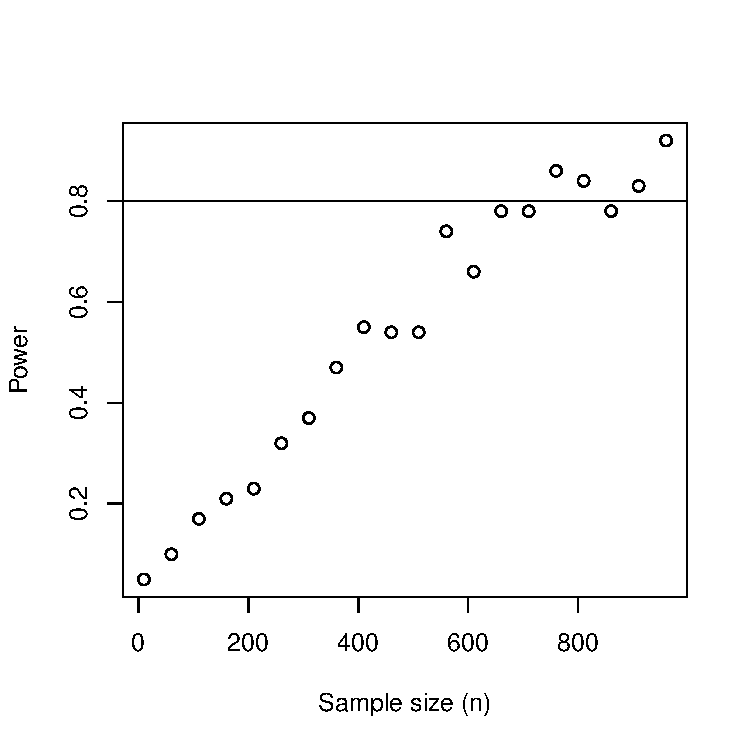
\includegraphics[width=\maxwidth]{figure/unnamed-chunk-7-1} 

\end{knitrout}

The plot shows that we need about 700-800 units to reach the commonly accepted power level of 0.8.

\end{document}
